\chapter[Referencial Teórico]{Referencial Teórico}

Para inicializar o nosso Referencial teórico de forma concisa em que se alinhe com o que foi proposto com o capítulo 1, é imprescindível abordar o contexto e papel da Fertilização In Vitro, qualidade dos embriões e desafios associados, além de evidenciar como a Inteligência Artificial aprimorar as taxas de sucesso de gravidez e minimiza os fatores de risco relacionados a abortos, problemas cromossômicos e reduzir os impactos emocionais e físicos associados a esses desafios.

\section{Fertilização In Vitro}

Registros históricos mostram que as civilizações antigas, como a grega que realizavam rituais e peregrinações para deidades e a egípcia que adotavam talismãs e amuletos para invocar bençãos dos deuses da fertilidade, deram uma grande importância à fertilidade, entendendo como uma bênção divina e continuação da linhagem da sociedade. Cada civilização possui métodos que buscavam a fertilidade, apesar de serem considerados como crenças em contraste com a ciência, ainda refletem que essa busca sempre foi um interesse enraizado nas culturas humanas \cite{moura2020}

Com o passar dos anos e da evolução do campo científico, essa busca pela fertilidade teve um avanço significativo na biologia e medicina. “A primeira inseminação artificial de que se tem registro foi realizada pelos árabes em 1332, em equino”, porém os primeiros resultados em seres humanos, com inseminação de sêmen no útero, foram obtidos apenas no final do século XVIII \cite{moura2020}. Dos anos 1970 em diante, essa técnica vem sendo bastante utilizada e toda essa trajetória de desenvolvimento corroborou para a revolução dos limites da concepção assistida, contribuindo cada vez mais as taxas de sucesso dessas reproduções assistidas.

A Reprodução Assistida (RA), depois de décadas sendo aprimorada, é definida como um “conjunto de técnicas, utilizadas por médicos especializados, que tem por finalidade facilitar ou viabilizar a procriação por homens e mulheres estéreis ou inférteis” \cite{souzamarise2024}. Ao citar o tema de reprodução assistida, é comum que venha à mente a Fertilização In Vitro (FIV).

A FIV é a técnica mais conhecida e mais complexa da RA. Ela promove a união, em ambiente laboratorial, do óvulo —célula reprodutiva feminina, também conhecida como gameta feminino— ao espermatozóide —célula reprodutiva masculina, ou gameta masculino— \cite{associacaobrasileira2024}. Em termos mais técnicos, é a coleta de um óvulo (ou ovócito) maduro, fertiliza-o em laboratório e transfere o embrião —fase inicial do desenvolvimento de um organismo após a fertilização, quando o óvulo e o espermatozóide se combinam— resultante para o útero.  O ano de 1978 foi marcado por uma grande evolução na medicina reprodutiva: o nascimento do primeiro bebê concebido pela FIV. Louise Brown, “o neném de proveta”, nasceu no Reino Unido, com a técnica de fertilizar um óvulo fora do corpo humano, realizada pelos médicos Patrick Steptoe e Robert Edwards \cite{corleta2010}. 

Após esse feito histórico, a medicina reprodutiva foi transformada e abriu novas oportunidades para pessoas que enfrentam essa dificuldade de fertilidade. Esses fatos citados destacam como, ao longo do tempo, a humanidade sempre procurou superar a infertilidade. Hoje, com a combinação dos avanços da medicina e da tecnologia, nos concede não apenas efetuar a fertilização in vitro, mas também realizar exames detalhados para descobrir a qualidade genética dos embriões, auxiliando ainda mais as taxas de sucesso da FIV. 

No próximo tópico, discutiremos a análise de embriões, procedimento esse que auxilia a identificar possíveis anomalias e aumentar as chances de concepção saudável, e a sua importância na seleção para a FIV.

\section{Métodos de Avaliação Genética em Reprodução Assistida}

Para evoluir na constatação de doenças genéticas na plore relacionadas ao número de cromossomos (Aneuploidia), são os métodos de avaliação genética em RA que fazem a análise para identificar possíveis anomalias, já que “a qualidade dos embriões é o fator mais crítico para o sucesso da fertilização in vitro” \cite{wang2019}, pois desempenham um papel expressivo para evitar os abortos, visto que estudos indicam que até 50\% de perdas gestacionais são devidas a anormalidades cromossômicas \cite{scienceofbiogenetics2024}. Após anos de pesquisa, o progresso na testagem genética vem permitindo cada vez mais diagnósticos precisos e técnicas mais avançadas, complexas e atreladas a tecnologia, como a Testagem Genética Pré-implantacional, conhecido como PGT.

Pelo final do século XX, o método do PGT começou a ser usado para realizar o rastreamento de doenças genéticas que possuíam uma alta taxa de incidência nas populações de amostra \cite{yang2024}. Com ele, foi propiciada a triagem de embriões antes da implementação, permitindo a seleção de embriões que possuíam menos riscos \cite{scienceofbiogenetics2024}. Atualmente, existem três tipos de PGT: “(1) para aneuploidia (PGT-A), como Síndrome de Down e Síndrome de Turner; (2) para defeitos monogênicos/gene único (PGT-M), como distrofia miotônica e fibrose cística; (3) e para rearranjos estruturais cromossômicos (PGT-SR)” \cite{yang2024}. Neste estudo, a atenção está voltada para a Testagem Genética Pré-implantacional para Aneuploidias (PGT-A), que distingue alterações no número de cromossomos dos embriões para melhorar a seleção embrionária com o objetivo de evitar a aneuploidia.  

O Dr. Bruno Ramalho explica que o PGT-A é um procedimento embrionário realizado em embriões durante as etapas de FIV que analisa o número de cromossomos em cada embrião antes de transferi-los, aumentando as porcentagens de uma transferência de FIV sucedida, garantindo que os embriões tenham o número correto de cromossomos. Também ressaltou que um embrião considerado “normal” (euploide), os mais desejados pois produzem a maior chance de uma gravidez bem-sucedida, possui 23 pares de cromossomos oriundos do esperma e 23 pares oriundos do óvulo, com um total de 46 cromossomos. O embrião considerado “anormal” (aneuploide) tem uma contagem a mais em algum cromossomo, assim, tendo 3 cópias, em oposição às duas que deveria ter \cite{cnyfertility2024}. Mas afinal, como o PGT-A performa? Explicaremos em 5 etapas para melhor entendimento:

\begin{itemize}
    \item \textbf{Etapa 1: Biópsia de tecido}
    \begin{itemize}
        \item Nessa primeira etapa de teste, é realizada depois dos estágios de estimulação ovariana—processo em que medicamentos hormonais são usados para estimular os ovários—, coleta de óvulos, fertilização e desenvolvimento embrionário em FIV. A partir do momento em que os embriões chegam em um estágio de desenvolvimento de aproximadamente 5 a 7 dias após a fertilização, é realizado uma biópsia—retirada de algumas células de um embrião—de tecido, com a consequência da retirada de uma amostra das células de cada embrião congelado para realizar testes genéticos \cite{cnyfertility2024}. 
    \end{itemize}

    \item \textbf{Etapa 2: Envio de amostras e congelamento de embriões}
    \begin{itemize}
        \item Após a etapa 1, essas amostras de tecido retiradas das células de cada embrião são enviadas para o laboratório de genética, é lá que se realizam os testes de verificação. Os embriões são congelados e armazenados até a hora da transferência do embrião selecionado \cite{cnyfertility2024}. 
    \end{itemize}

    \item \textbf{Etapa 3: Análise cromossômica PGT-A}
    \begin{itemize}
        \item Depois que as amostras de tecido chegarem no laboratório e da análise dos cromossomos, o PGT-A é concluído. Na análise, os embriões passam por exames relacionados a anormalidades cromossômicas \cite{cnyfertility2024}. 
    \end{itemize}

    \item \textbf{Etapa 4: O Relatório Genético}
    \begin{itemize}
        \item Ao concluir a análise, o laboratório envia um relatório genético que tem os detalhes dos status de cada embrião selecionado para teste, contendo nesse documento o número de cromossomos de cada. O médico especialista em fertilidade conferirá os resultados e relatará os resultados obtidos com o paciente em questão \cite{cnyfertility2024}. 
    \end{itemize}

    \item \textbf{Etapa 5: Seleção de embriões e transferência congelada}
    \begin{itemize}
        \item Se baseando nos resultados detalhados no relatório genético, o especialista em fertilidade escolherá o(s) embrião(ões) saudável(eis) para a transferência. O(s) embrião(ões) selecionado(s) será(ão) então descongelado(s) e preparado(s) quando for a hora da transferência do embrião \cite{cnyfertility2024}. 
    \end{itemize}
\end{itemize}

O resultado que o PGT-A entrega para pacientes que o utilizam é a classificação dos embriões, dentro dessa classificação existem 3 tipos de resultado diferentes para cada embrião. Eles são classificados com um dos três resultados potenciais do teste: Euplóide (normal)—todas as células amostradas do embrião têm 46 cromossomos—, mosaico (parcialmente normal, parcialmente anormal) —algumas células que foram testadas no embrião são normais, algumas são anormais—e aneuplóide (anormal) —todas as células obtidas da biópsia tinham um número anormal de cromossomos—\cite{cnyfertility2024}.

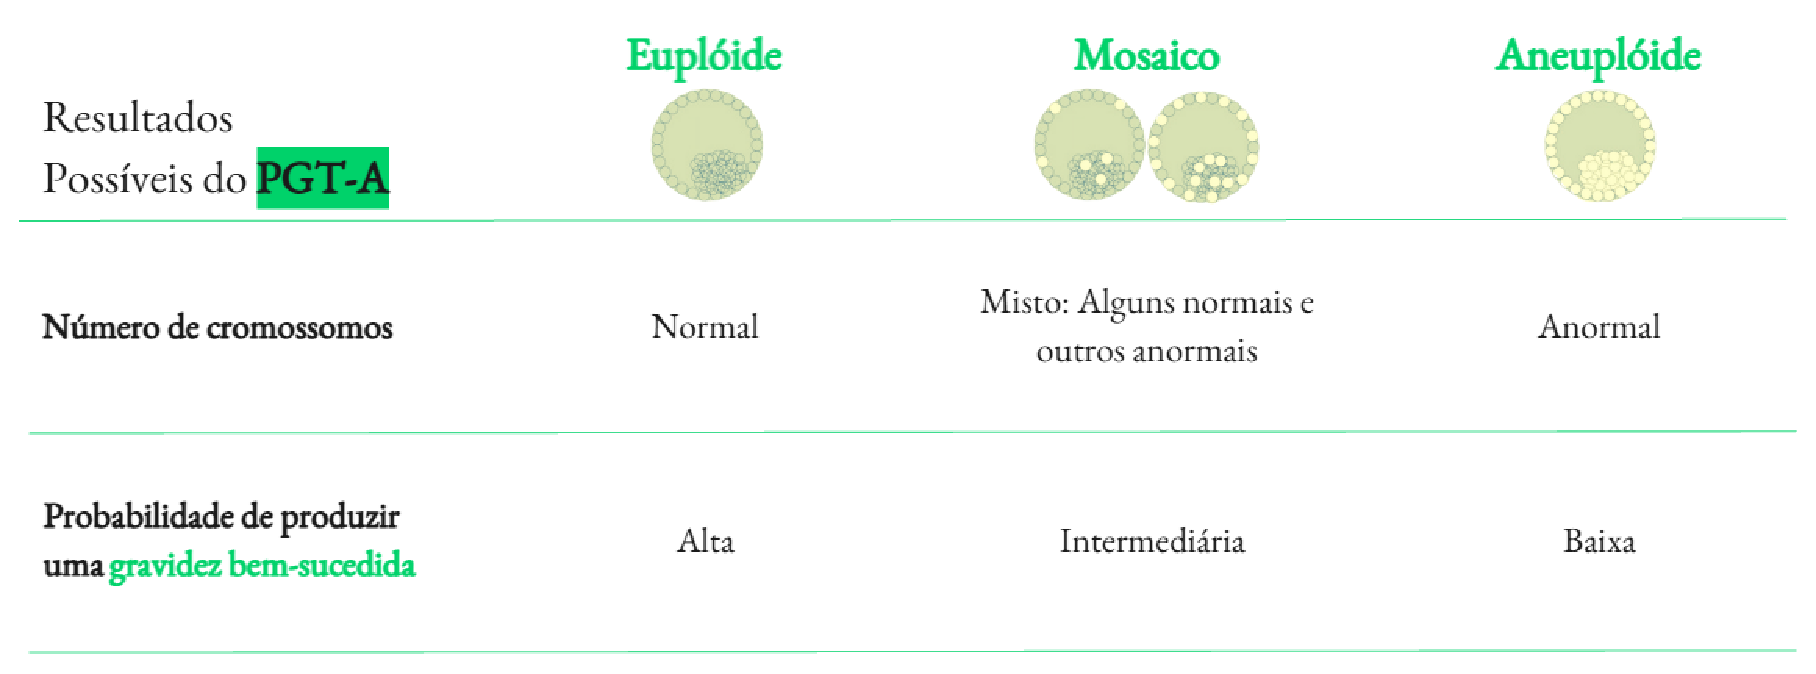
\includepdf{figuras/ResultadosPGT.pdf}

% \begin{figure}[h]
%     \centering
%     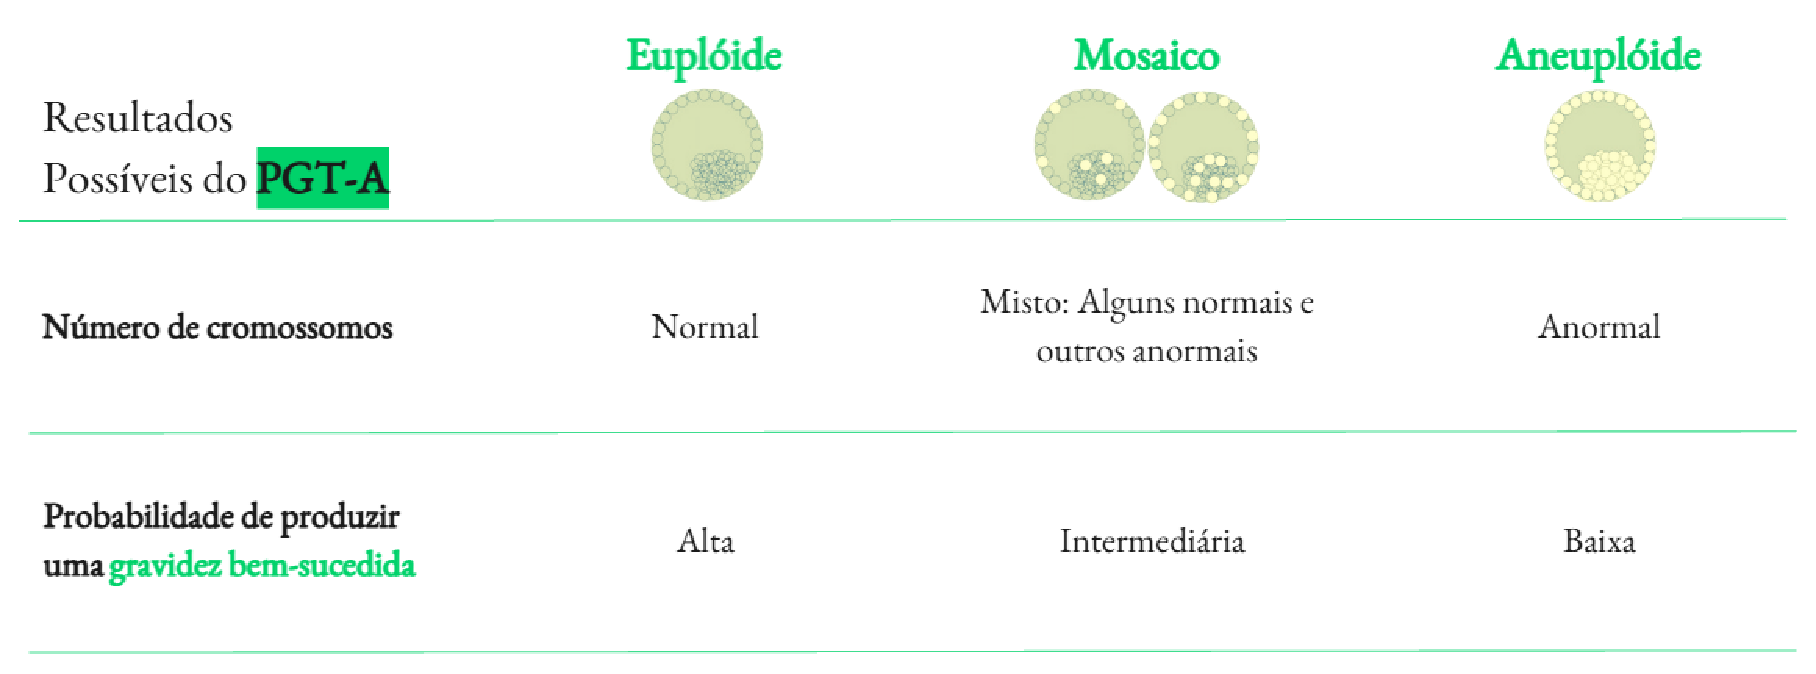
\includepdf[pages=-]{figuras/ResultadosPGT.pdf}
%     \caption{Imagem criada se baseando na imagem feita pela CNY Fertility em 2024. Essa imagem exibe um resumo dos possíveis resultados do PGT-A em embriões - CNY Fertility}
%     \label{resultado_pgt}
% \end{figure}

Dessa forma, é investigado qual é o melhor embrião entre os selecionados para a análise genética, tudo partindo de uma biópsia, como descrito na etapa 1. O PGT é um procedimento relativamente complexo pois exige uma biópsia dos embriões, onde qualquer dano mínimo deve ser evitado e por esse motivo é considerado um método invasivo e apresenta riscos potenciais ao embrião \cite{yang2024}.

Um método invasivo na FIV são aqueles que utilizam técnicas de operação direta no embrião ou em células que vão formar o embrião. Um exemplo é a biópsia citada nas etapas do PGT-A, em que se realiza uma remoção da célula do embrião para analisar geneticamente, \citeonline(phillips2024) levantam aflições de que a remoção dessas células em crescimento possa impedir o desenvolvimento do embrião em questão, comprometendo os resultados neonatais, pois as técnicas de micromanipulação para biópsia não são totalmente isentas de riscos, como citado por \citeonline(leaver2019). “Além disso, a natureza invasiva da biópsia requer uma manipulação de embriões demorada por embriologistas experientes, tornando este um procedimento caro para os pacientes” \cite{phillips2024; leaver2019}. Ainda que o PGT-A permita detectar aneuploidias e expandir as porcentagem de gravidez bem-sucedida, se tem a chance de afetar o potencial de implantação do embrião. Por esses motivos apresentados, métodos não-invasivos estão sendo estudados para disponibilizar alternativas eficientes e seguras, se tornando cada vez mais significativas. Um exemplo de técnica não-invasiva é o Time-Lapse System – Sistema de Time-Lapse (TLS).

O TLS é uma técnica que “requer tirar fotos contínuas dos embriões em crescimento em intervalos consistentes, sem interferir no ambiente de sua cultura” \cite{moustakli2024}. De acordo com o Dr. Bruno Ramalho, o especialista em fertilidade podem utilizar essa técnica para monitorar o momento das divisões celulares e regularidade disso, observando momentos importantes do crescimento e, com esse monitoramento contínuo, conseguindo distinguir um embrião euplóide ou aneuplóide de acordo com seu padrão desenvolvimento. De acordo com \citeonline(moustakli2024), o TLS dispõe-se oferecer insights valiosos sobre a saúde e o potencial de desenvolvimento dos embriões, utilizando técnicas não invasivas como a biópsia de embriões. “De fato, alguns autores demonstram que a TLS e as pontuações morfocinéticas podem melhorar a implantação e as taxas de gravidez clínica em comparação com os métodos convencionais” \cite{boucret2021}.

Os dados morfocinéticos de embriões coletados pelo TLS oferecem uma oportunidade para melhorar a escolha de embriões em tratamentos de FIV. Supondo uma IA que tem a capacidade de analisar esses dados, teríamos a possibilidade de identificar padrões e predizer a porcentagem, de euploidia. Isso representaria uma abordagem não-invasiva e mais acessível financeiramente. Ao pensar nessa IA e esse ser o objetivo do trabalho presente, é imprescindível compreender como a IA poderia ser aplicada nesse contexto e como ela poderia ser capaz de fazer essa abordagem. 

\section{Inteligência Artificial}

Com a chegada dos computadores modernos após a Segunda Guerra Mundial, abriu-se a possibilidade de desenvolver programas capazes de executar tarefas acadêmicas complexas \cite{jeffery2022}. Esse avanço, aliado a novas descobertas na área da neurociência, levou cientistas a considerar a criação de um "cérebro eletrônico", ideia que eventualmente se transformaria no conceito de inteligência artificial \cite{jeffery2022}. Não existe, ainda, uma definição  única e amplamente aceita do que seria Inteligência Artificial \cite{sheikh2023}. Pode-se dizer que IA significa a imitação por computadores da inteligência inerente aos humanos \cite{sheikh2023}, ou seja, elas não são apenas programadas para executar tarefas, mas sim para simular habilidades humanas, como o pensamento e o raciocínio. Essa definição, no entanto, é ampla e possui limitações, já que explica somente o termo “inteligência artificial” em outras palavras. 

As dificuldades em definir IA não são, portanto, o resultado de alguma deficiência ou descuido, mas surgem do fato de que fomos incapazes de determinar precisamente qual inteligência desejaríamos replicar artificialmente \cite{sheikh2023}. Dessa forma, definimos a Inteligência Artificial como sistemas que exibem comportamento inteligente ao analisar seu ambiente e tomar ações – com algum grau de autonomia – para atingir objetivos específicos \cite{sheikh2023}.

As aplicações práticas da IA abrangem áreas como finanças, veículos autônomos, diagnóstico médico, reconhecimento de imagem e voz, entre outras. Em particular, na medicina reprodutiva, a IA tem se mostrado promissora na melhoria de processos como a fertilização in vitro (FIV). Assim, essa busca por imitar a inteligência humana e entender seus processos cognitivos levou ao desenvolvimento de diversas abordagens, entre elas o Aprendizado de Máquina (Machine Learning, ML)

Aprendizado de Máquina, subconjunto da IA,  envolve a capacidade de computadores de interpretar grandes volumes de dados, construir modelos baseados nesses dados e, assim, gerar hipóteses ou previsões sobre o mundo ao seu redor \cite{russell2016}. Nesse caso, a ML está sendo expandida para vários setores, como na medicina, a qual algoritmos podem ser treinados para reconhecer padrões genéticos em embriões e classificar o melhor embrião para implantação e, a partir disso, prever essas questões em novos embriões. Os métodos de ML são geralmente classificados em três tipos principais: aprendizado supervisionado, aprendizado não supervisionado e aprendizado por reforço.

\subsection{Aprendizado Supervisionado}

O aprendizado supervisionado é uma das abordagens mais comuns em inteligência artificial e consiste no treinamento de algoritmos com base em conjuntos de dados rotulados. sso significa que o algoritmo recebe como entrada um conjunto de dados em que as variáveis de entrada (inputs) e os resultados esperados (outputs) já são conhecidos, permitindo que ele aprenda a correlacioná-los de forma eficiente \cite{russell2016}. O processo consiste em alimentar o algoritmo com esses dados rotulados, ajustar os parâmetros do modelo com base nas diferenças entre as previsões e os resultados reais, e repetir o ciclo até que o desempenho seja satisfatório e preciso \cite{trask2019}. 

Uma técnica amplamente usada dentro do aprendizado supervisionado é a classificação, cujo objetivo é atribuir rótulos ou classes pré-definidas aos dados. Para isso, o algoritmo é treinado com um conjunto de exemplos conhecidos, onde cada entrada está associada à sua respectiva classe. O modelo aprende, então, a identificar padrões ou características que distinguem essas classes \cite{izbicki2020}. No contexto da medicina reprodutiva, por exemplo, um modelo de classificação pode ser treinado com dados rotulados que diferenciam embriões euploides e aneuploides. Dessa forma, o algoritmo aprende a reconhecer características comuns a cada grupo e pode prever a probabilidade de um novo embrião pertencer a uma dessas categorias.

De maneira geral, um algoritmo de aprendizado supervisionado separa o banco de dados, seja de forma aleatória ou pré-definida, em três subconjuntos: treinamento, validação e teste (Izbicki, 2020). Na primeira etapa, chamada de fase de treinamento, o algoritmo é ajustado para identificar padrões nos dados de entrada e associá-los às classes desejadas \cite{izbicki2020}. Em seguida, na fase de validação, utiliza-se outro subconjunto de dados, que não foi usado no treinamento, para avaliar o desempenho do modelo, comparando suas previsões com as respostas corretas \cite{izbicki2020}. Se os resultados não forem satisfatórios, os hiperparâmetros – parâmetros que orientam o processo de treinamento – devem ser ajustados, e o banco de dados é reorganizado e dividido novamente, repetindo-se as duas etapas iniciais \cite{izbicki2020}. Após obter um resultado satisfatório, aplica-se o conjunto de testes para mensurar métricas como acurácia, recall, precisão, entre outros, garantindo o desempenho esperado da IA \cite{izbicki2020}.

Uma boa prática para a escolha das amostras que compõem os conjuntos de treinamento e validação é fazê-la de maneira aleatória \cite{izbicki2020}. Neste procedimento, utiliza-se um gerador de números aleatórios para selecionar quais amostras farão parte do treinamento e quais serão destinadas à validação e teste \cite{izbicki2020}. Essa abordagem evita problemas decorrentes de bancos de dados previamente ordenados com base em alguma variável, como quando as observações são organizadas em função de uma característica específica durante a coleta. A aleatoriedade garante que o modelo tenha uma visão mais representativa e imparcial dos dados disponíveis \cite{izbicki2020}.

Diferente do aprendizado supervisionado, o aprendizado não supervisionado não depende de dados rotulados. Ele explora hipóteses de correlações e relacionamentos entre eles para identificar padrões ou estruturas ocultas, agrupando os dados com base em semelhanças (clustering) ou identificando anomalias \cite{russell2016; trask2019}. Já o aprendizado por reforço é inspirado no processo de tentativa e erro do aprendizado humano. Nesse tipo de aprendizado,  o algoritmo interage com o ambiente, experimenta diferentes ações e recebe feedback positivo ou negativo em função dos resultados alcançados. Com o tempo, o modelo aprende a otimizar suas decisões para alcançar um objetivo final, mesmo sem um conjunto de dados pré-definido \cite{risala2023}.

Neste trabalho, utilizaremos o aprendizado supervisionado, mais especificamente técnicas de classificação, para abordar o problema proposto. Essa escolha é motivada pela necessidade de analisar dados rotulados e prever categorias específicas com alta precisão, características intrínsecas dessa abordagem.

\section{Identificação de Padrões Morfocinéticos e Predição de Euploidia com IA e Trabalhos Correlatos}

Os dados que são coletados pela tecnologia do TLS, são chamados de “dados morfocinéticos”, que são definidos como “dados do desenvolvimento dos embriões” \cite{oliveira2024}. Essa informação reunida proporciona noções detalhadas sobre o padrão do desenvolvimento e divisão celular embrionário. Atualmente, após recorrentes estudos em cima desses dados, sabe-se que as “características morfocinéticas dos embriões têm sido associadas à avaliação de sua potência de desenvolvimento”, ou seja, se um embrião analisado pelo TLS tenha um melhor desenvolvimento, ele terá mais probabilidade de ser euplóide, pois um bom desempenho de um embrião é capaz de prever a implantação \cite{yuan2023}.

Os modelos de TLS, de acordo com \citeonline(yuan2023), tem uma avaliação contínua na etapa do desenvolvimento embrionário por meio de suas imagens e, por observações estáticas, monitora as características do embrião, como tempo e padrões de divisão celular, fornecendo uma base para prever a euploidia. O TLS por si só, não opera com a IA, mas é frequentemente mesclado com essa tecnologia para maiores análises. Um exemplo é o estudo do \citeonline(yuan2023), o artigo “Development of an artifcial intelligence based model for predicting the euploidy of blastocysts in PGT‐A treatments” teve como objetivo utilizar o TLS e desenvolver um modelo de IA usando uma técnica de regressão logística, para predizer a euploidia de blastocistos—fase do desenvolvimento embrionário que ocorre após a clivagem do óvulo fertilizado—em tratamentos de PGT-A, ajudando a identificar embriões com maiores possibilidades de serem geneticamente normais antes da etapa de transferência. O modelo foi avaliado com uma boa precisão, indicando que ele consegue distinguir entre embriões euploides e aneuploides.

Outro estudo é o de \citeonline(souzarebeca2022), “Análise da ploidia de embriões humanos por meio da inteligência artificial com o uso de variáveis de morfologia, morfocinética e variáveis relacionadas com a paciente”, também descreve o uso de IA para fazer a predição da ploidia de embriões, classificando os embriões como euplóides e aneuplóides. Para realizar isso, o estudo também combinou dados morfológicas, morfocinéticas e parâmetros clínicos, como o \citeonline(yuan2023). O modelo utilizado por \citeonline(souzarebeca2022)foi uma rede neural artificial (RNA), treinada justamente para classificar os embriões como citado.

Divergente do trabalho de “Zhenya Yuan, Mu Yuan, Xuemei Song, Xiaojie Huang e WeiqiaoYan” \cite{yuan2023} e da de “Rebeca Colauto Milanezi de Souza” \cite{souzarebeca2022}, que possuem o objetivo de fazer uma previsão binária de euploidia (mostrando se o embrião em estudo é euploide ou não), o modelo que propomos realizar neste trabalho em questão visa prever a porcentagem de aneuploidia. Com essa diferença de resultado, permitimos uma avaliação mais específica da saúde genética do embrião analisado, ofertando um indicador quantitativo em vez de uma classificação binária.

Para fazer a predição da porcentagem de euploidia, planejamos [citar o modelo de IA que iremos fazer], visando otimizar a precisão da predição, enquanto o modelo dos artigos usam uma técnica de regressão logística voltada em previsões binárias.

Com essas diferenças citadas, temos o objetivo de criar uma alternativa menos invasiva e mais acessível para a seleção de embriões na FIV.










